% !TeX spellcheck = en_GB
\documentclass[a4paper,11pt]{article}

\usepackage[a4paper]{geometry}
\usepackage[english]{babel}
\usepackage{amsmath}
\usepackage{amsbsy}
\usepackage{libertine}
\usepackage{parskip}
\usepackage{booktabs}
\usepackage[usenames,dvipsnames,svgnames,table]{xcolor}
\usepackage{makecell}
\usepackage{hyperref}
\usepackage{siunitx}
\usepackage{graphicx}
\usepackage{float}
\hypersetup{pdftitle={The Definitive Physics Definition List},pdfauthor={Engineers of Dubious Quality},bookmarksnumbered=true,bookmarksopen=true,bookmarksopenlevel=1,colorlinks=true,allcolors=black,pdfstartview=Fit,pdfpagemode=UseOutlines,pdfpagelayout=TwoPageRight}

\newlength{\oldparskip}
\setlength{\parskip}{2ex plus 0.5ex minus 0.2ex}

\newcolumntype{L}[1]{>{\raggedright\let\newline\\\arraybackslash\hspace{0pt}}p{#1}}
\newcolumntype{C}[1]{>{\centering\let\newline\\\arraybackslash\hspace{0pt}}p{#1}}
\newcolumntype{R}[1]{>{\raggedleft\let\newline\\\arraybackslash\hspace{0pt}}p{#1}}

\title{The Definitive Physics Definition List}
\author{Engineers of Dubious Quality\\Yudong, Yicheng, Samuel, and Walter}

\begin{document}
	
	\maketitle
	
	\section{Measurements}
	Express errors/uncertainties to 1 s.f. and write the measured value to the same decimal place as its error/uncertainty
	
	\begin{center}
		\renewcommand{\arraystretch}{1.5}
		\begin{tabular}{@{} l p{11.6cm} @{}}
			\toprule
			Systematic Error & An error that occurs consistently more or consistently less than the actual reading.\\
			Random Error & An error that occurs as a scattering (or spreading) of readings about the average or mean value of the measurements. \\
			\midrule
			Precision & The \textbf{reproducibility} of a measurement. Repeated measurements which are very close to one another are precise measurements. Thus an experiment which has \textbf{small random errors} (i.e. small spread of readings) is said to have \textbf{high precision}. \\
			Accuracy & The \textbf{agreement} between the measured value and the true or accepted value of a quantity. An experiment which has \textbf{small systematic errors} is said to have \textbf{high accuracy}. The \textbf{average value} is close to the true value. \\
			\midrule
			Vector Quantity & A quantity that has a \textbf{magnitude and direction}. \\
			Scalar Quantity & A quantity that has a \textbf{magnitude only}. \\
			\bottomrule
		\end{tabular}
	\end{center}
	\newpage
	\section{Kinematics}
	We define a coordinate system with defined reference positive directions, and we assume constant acceleration when we apply the kinematics equations.
	\begin{center}
		\renewcommand{\arraystretch}{1.5}
		\begin{tabular}{@{} l l p{9.1cm} @{}}
			\toprule
			Displacement & $\textbf{s}$ & The distance travelled in a stated direction from a reference point. \\
			Velocity & $\displaystyle \textbf{v} = \frac{d\textbf{s}}{dt}$ & The rate of change of displacement with respect to time.\\
			\rule{0pt}{20pt}Speed & $\displaystyle v=\left|\textbf{v}\right| = \left|\frac{d\textbf{s}}{dt}\right|$ & The rate of change of distance travelled with respect to time. \\
			\rule{0pt}{20pt}Acceleration &  $\displaystyle \textbf{a} = \frac{d\textbf{v}}{dt} = \frac{d^2\textbf{s}}{dt^2}$ & The rate of change of velocity with respect to time. \vspace{4mm}\\
			\bottomrule
		\end{tabular}
	\end{center}
	
	\section{Dynamics}
		\subsection{Newton's Laws of Motion}
			\oldparskip=\parskip
			\begin{center}
				\renewcommand{\arraystretch}{1.2}
				\begin{tabular}{@{} l >{\parskip=\oldparskip}p{11.5cm} @{}}
					\toprule
					1\textsuperscript{st} Law & A body will continue in its \textbf{state of rest}, or \textbf{move} at \textbf{constant speed in a straight line} unless an \textbf{external resultant force} acts on it.\\
					$\rightarrow$ Inertia & The resistance to change in the state of motion of an object \\
					$\rightarrow$ Mass & A property of that determines the objects inertia. \\
					\midrule
					2\textsuperscript{nd} Law & The \textbf{rate of change of linear momentum} of a body is \textbf{directly proportional} to the resultant force acting on it, and its direction is in the \textbf{same direction} as this resultant force. \par The \textbf{force acting on an object} is defined as the \textbf{rate of change of linear momentum} of an object. $$\textbf{F} \propto \frac{d\textbf{p}}{dt}, ~\textbf{F}=m\textbf{a} \textrm{ (if constant mass)} \vspace*{-\baselineskip}$$ \\
					\midrule
					3\textsuperscript{rd} Law & If body A exerts a force on body B, then body B will exert an \textbf{equal and opposite} force on body A. \par \textit{Note:} Action-Reaction Pairs act on different bodies and are of the same nature.\\
					\midrule
					Weight & The gravitational force acting on the object. \\
					Weightlessness & There is no contact force acting on the object. \textit{A body experiences apparent weightlessness when the resultant force acting on it is its weight, or it is undergoing freefall.} \\
					\bottomrule
				\end{tabular}
			\end{center}
		\subsection{Momentum}
			\begin{center}
				\renewcommand{\arraystretch}{1.2}
				\begin{tabular}{@{} p{2.7cm} l p{6.8cm} @{}}
					\toprule
					Linear Momentum & $\textbf{p}=m\textbf{v}$ & The product of an object's mass and its velocity. \\
					\rule{0pt}{20pt}Impulse & $\displaystyle \textbf{J}=\int_{t1}^{t2}\textbf{F}~dt=\textbf{p}_{f}-\textbf{p}_{i}$	& The product of the average force acting on an object and the time interval that the force is being applied.\\	
					\midrule
					Principle of Conservation of Linear Momentum & \multicolumn{2}{p{10.7cm}}{The total momentum of the system is a constant when no external resultant force acts on it.}\\
					\bottomrule
				\end{tabular}
			\end{center}
	\section{Forces}
		\begin{center}
			\renewcommand{\arraystretch}{1.2}
			\begin{tabular}{@{} l l p{7cm} @{}}
				\toprule
				Pressure due to Fluid & $\Delta P = h\rho g$ & The force acting per unit area by the fluid on a body submerged at a depth in the fluid. \\
				Upthrust & $U=m_{f}g=\rho V_{dis}g$ & The \textbf{net upward force exerted by a fluid} on a body partially or fully submerged in the fluid. \\
				Principle of Floatation & $mg=U=\rho V_{dis} g$ & This holds true for an object floating in equilibrium in a fluid.  \\
				Drag & \multicolumn{1}{p{2.5cm}}{$\textbf{F}_{\textbf{D}}=k\textbf{v}$ \par (Laminar Flow)} & It is the force resisting an object \textbf{moving relative to a fluid}. It always \textbf{opposes} motion, and its magnitude is \textbf{dependent on the velocity} of the object.\\
				\midrule
				Moment of a force (Torque) & $\boldsymbol{\tau}=\textbf{r} \times \textbf{F}$ & Moment of a force about a point (the pivot) is the \textbf{product} of the magnitude of the force and the \textbf{perpendicular distance} of the \textbf{line of action} of the force to the point. \\
				Couple & \multicolumn{2}{p{10.3cm}}{A couple always consists of 2 parallel forces which are equal in magnitude and opposite in direction (their lines of action do not coincide)} \\
				Torque of a couple & \multicolumn{2}{p{10.3cm}}{The \textbf{product} of the \textbf{magnitude of one of the forces} of the couple and the \textbf{perpendicular distance between the forces.}} \\
				Center of gravity of a body & \multicolumn{2}{l}{It is the point at which the weight of the body appears to act.} \\
				\bottomrule
			\end{tabular}
		\end{center}
		\subsection{Equilibrium of Forces}
			For a rigid body to be in static equilibrium, 2 conditions must be satisfied:
			
			\begin{tabular}{@{} C{0.48\textwidth} C{0.48\textwidth}  @{}}
				1. \textbf{Translational equilibrium} \par The \textbf{net external} force acting on the body is zero. $$\sum F = 0$$ & 2. \textbf{Rotational Equilibrium} \par The \textbf{net torque} on the body about \textbf{\underline{ANY} point} is zero. $$\sum \tau = 0$$ \vspace*{-\baselineskip} \\
			\end{tabular}
			\vspace{-\baselineskip}
			\begin{center}
				\renewcommand{\arraystretch}{1.2}
				\begin{tabular}{@{} l p{10.8cm} @{}}
					\toprule
					Principle of Moments & The principle of moments states that when in (rotational) equilibrium the total sum of the anti-clockwise moment is equal to the total sum of the clockwise moment. \\
					\bottomrule
				\end{tabular}
			\end{center}
			
			For a 3-forces system in static equilibrium, the 3 forces form \textit{a closed vector triangle}. For 3 forces acting on an \textit{extended body} in static equilibrium, the lines of action of the 3 forces \textit{must intersect at a common point} unless the 3 forces are parallel.

	\section{Work, Energy, and Power}
		\begin{center}
			\renewcommand{\arraystretch}{1.5}
			\begin{tabular}{p{4cm} l >{\parskip=\oldparskip}p{7.7cm} @{}}
				\toprule
				Principle of Conservation of Energy & \multicolumn{2}{p{10.7cm}}{Energy can be \textbf{converted} from one form to another, but it \textbf{cannot be created or destroyed}. The \textbf{total energy} of an \textbf{isolated} system is constant}\\
				\midrule
				Work done by a Force & $\displaystyle W=\int_{C}^{} \textbf{F} \cdot d\textbf{s} $ & The product of the magnitude of the force $F$ and the displacement $s$ in the direction of the force. \\
				Total Mechanical Energy & $\sum \textrm{KE} + \sum \textrm{PE}$ & The total mechnical energy of a system is the sum of all types of kinetic energy and potential energy. \\
				Kinetic Energy & $E_k = \frac{1}{2}mv^2$ & Kinetic energy of a body is a measure of the energy possessed by the body by virtue of its motion.\\
				Potential Energy & --- & The amount of work that was done on a body to give it that position. \par It is a measure of the energy possessed by the body by virtue of its position or the arrangement of the system that it is part of. [There are 3 types: Elastic, Gravitational and Electrical]\\
				Power & $\displaystyle P=\frac{dW}{dt}=Fv$ & Power is the rate at which work is done. \par When a force acts on a body that is moving with velocity $v$, in the direction of the force, it delivers power to the body at the rate given by $P=Fv$.\\
				\bottomrule
			\end{tabular}
		\end{center}
	\newpage
	\section{Circular Motion}
		Always write ``The \underline{\hspace{1.5cm}} forces provide the centripetal force".
		\begin{center}
			\renewcommand{\arraystretch}{1.5}
			\begin{tabular}{@{} l l p{7cm} @{}}
				\toprule
				Angular Displacement & $\theta$ & Angle swept from a reference point. \\
				Angular Velocity & $\displaystyle \omega=\frac{d\theta}{dt}=\frac{2\pi}{T}=2\pi f$ & Rate of change of angular displacement with respect to time. \\
				Period & $\displaystyle T=\frac{1}{f}$ & Time taken for one complete revolution. \vspace{\baselineskip}\\
				Linear/Tangential Speed & $\displaystyle v=\frac{2\pi r}{T}=r\omega$ & \textit{(No need to know definition)}\vspace{\baselineskip}\\
				\bottomrule
			\end{tabular}
		\end{center}
		\subsection{Uniform Circular Motion}
			Conditions: $\omega$ constant, $r$ constant
			\begin{center}
				\renewcommand{\arraystretch}{1.5}
				\begin{tabular}{@{} p{4cm} p{10.6cm} @{}}
					\toprule
					Uniform Circular Motion & It is the motion of an object travelling at constant (uniform) speed in a circular path. \\
					Centripetal Acceleration/ \par Centripetal Force& The centripetal acceleration/force is directed \textbf{radially inward} towards the centre of the circular path. The direction of the centripetal acceleration/force is continuously changing. $$\sum a = a_{net} = a_c=\frac{v^2}{r}=r\omega^2=v\omega$$ No acceleration/force in the tangential direction. $\Rightarrow$ No work done. 
					\\
					\bottomrule
				\end{tabular}
			\end{center}
	\newpage
	\section{Gravitation}
	The `G's in the following left column stands for `Gravitation', or `Gravitational'.
		\begin{center}
			\renewcommand{\arraystretch}{1.6}
			\begin{tabular}{@{} l l p{7.8cm} @{}}
				\toprule
				Newton's Law of G & $\displaystyle F_g = G\frac{m_1 m_2}{r^2}$ & Gravitational force between 2 objects is \textbf{directly proportional} to the product of their masses, and \textbf{inversely proportional} to the square of the distances between them. \\
				G Field Strength & $\displaystyle g = \frac{F_g}{m} = G\frac{M}{r^2}$ & The GFS $g$ at a point in a gravitational field is the \textbf{gravitational force per unit mass} acting on a small mass placed at that point. \\
				G Field & --- & A region of space surrounding a body possessing mass, in which any other body that has mass will experience a force of attraction.\\
				G Potential & \multicolumn{1}{p{2.8cm}}{$\displaystyle \phi = \frac{U}{m} = -G \frac{M}{r}$ \par \vspace{1.5mm} $\displaystyle g=-\frac{d\phi}{dr}$\vspace{1.5mm}} & Work done per unit mass by an external force in bringing a small mass from infinity to that point in a gravitational field without a change in kinetic energy.\\
				G Potential Energy & \multicolumn{1}{p{2.6cm}}{$\displaystyle U = -G \frac{m_1 m_2}{r}$ \par \vspace{2mm} $\displaystyle F_g=-\frac{dU}{dr}$} & Work done by an external force in bringing a mass from infinity to that point in a gravitational field without a change in kinetic energy. \\
				Geostationary Orbit & & A satellite in orbit that appears stationary to an observer on Earth. It has a period of \SI{24}{\hour}, orbits the Earth along the plane containing the equator, and moves from the West to the East.\\
				\bottomrule
			\end{tabular}
		\end{center}
	\newpage
	\section{Oscillations}
		\begin{center}
			\renewcommand{\arraystretch}{1.2}
			\begin{tabular}{@{} l l p{8cm} @{}}
				\toprule
				Simple Harmonic Motion & $a=-\omega^2x$ & A body \textbf{oscillating} with SHM has \textbf{acceleration} that is \textbf{directly proportional} to the \textbf{displacement from equilibrium} and the acceleration is in a \textbf{direction opposite} to that of displacement from equilibrium. \\
				\bottomrule
			\end{tabular}
		\end{center}
		\subsection{Types of Oscillations}
			\begin{center}
				\renewcommand{\arraystretch}{1.6}
				\begin{tabular}{@{} l p{10.9cm} @{}}
					\toprule
					Damped Oscillation  & Oscillation in which the  \textbf{amplitude} of the oscillations \textbf{decreases with time}. \\
					$\rightarrow$ Light & In a lightly damped system, the total energy of the system decreases with time as energy is dissipated when the system oscillates against resistive forces. The amplitude of the system usually decreases \textit{exponentially} with time.\\
					$\rightarrow$ Critical & The system is said to be critically damped when it returns to the equilibrium position in the shortest possible time without oscillating at all. \\
					$\rightarrow$ Heavy & The system is said to be \textit{overdamped} if the oscillator takes a very long time to return to it equilibrium position.\\
					Forced Oscillation &  An oscillation under the influence of an \textbf{external periodic} force is called a forced oscillation.\\
					Resonance & Phenomenon where the \textbf{maximum amplitude} of an object driven to oscillate is achieved when the \textbf{driver frequency} is equal to the \textbf{natural frequency} due to efficient transfer of energy. \\
					\bottomrule
					\end{tabular}
			\end{center}
	\section{Waves and Superposition}
	\begin{center}
		\renewcommand{\arraystretch}{1.5}
		\begin{tabular}{@{} l p{10cm} @{}}
			\toprule
			Progressive Waves & Disturbance/Vibration which \textbf{propagates}, carrying \textbf{energy without physically transferring} the wave particle. \\
			$\rightarrow$ Transverse Waves & Progressive wave in which particles or fields oscillate perpendicular to direction of wave propagation. \\ 
			$\rightarrow$ Longitudinal Waves & Progressive wave in which particles oscillate parallel to direction of wave propagation. \\
			Intensity & Power per unit area $$E \propto A^2 \Rightarrow I \propto A^2$$ \vspace*{-\baselineskip}\\
			Polarisation & Vibrations in a transverse waves are restricted to only 1 direction in a plane normal to the direction of energy transfer. \\ 
			Principle of Superposition & When 2 or more waves of the \textbf{same type} superimpose, the \textbf{displacement} of a \textbf{resultant wave at any point at any instant} is the \textbf{vector sum} of the displacements of the individual waves at that point at that instant.\\
			Stationary/Standing Waves & Formed when 2 \textbf{similar} waves of \textbf{same speed, frequency and amplitude} travelling towards each other in \textbf{opposite} directions superimpose. \\
			Interference & The overlap of 2 or more waves to give a resultant wave whose displacement at every point at any time is given by the Principle of Superposition. \par $\Rightarrow$ Conditions: (i) Same kind of waves; (ii) overlap\\
			$\rightarrow$ Observable Interference & 
			\begin{minipage}[t]{\textwidth}%
				\begin{itemize}
					\item Same type, overlap
					\item Coherence 
					\item Roughly same Amplitude 
					\item Unpolarised or polarised in the same plane 
				\end{itemize}
			\end{minipage} \par 
			\underline{Constructive}: Oscillation at that point has maximum resultant amplitude and maximum intensity.\par
			\underline{Destructive}: Oscillation at that point has minimum resultant amplitude and minimum intensity.\\
			Diffraction & Spreading of waves into \textbf{``geometrical" shadow} after passing through an aperture or around an obstacle as a result of a \textbf{redistribution of energy}. \\
			\bottomrule
		\end{tabular}
	\end{center}
	\newpage
	\section{Thermal Physics}
		\begin{center}
			\renewcommand{\arraystretch}{1.5}
			\begin{tabular}{@{} l l p{8.5cm} @{}}
				\toprule
				Temperature & $T$ & Measure of the average kinetic energy the molecules in a system possess. \\
				Heat & $Q$ & Thermal energy that naturally flows from regions of higher to lower temperature. \\
				Thermal Equilibrium & & 2 objects in thermal contact with no net exchange of heat. \\
				Kelvin Scale & & Absolute temperature scale independent of thermometric properties. \\
				Absolute Zero & 0K & All molecules possess minimal internal energy. \\
				Specific Heat Capacity & $C$ & Amount of thermal energy per unit mass to increase the temperature of the unit mass of substance by one unit of temperature. \\
				Specific latent heat of fusion & $L_f$ & Amount of \textbf{thermal energy per unit mass} to convert the substance from solid to liquid without any change in temperature. \\
				Specific latent heat of vaporisation & $L_v$ & Amount of \textbf{thermal energy per unit mass} to convert the substance from liquid to gas without any change in temperature. \\
				Internal Energy & $U$ & Sum of microscopic random kinetic energy and microscopic potential energy of molecules in system. For ideal gases: $$U=\frac{3}{2}~nRT$$ \vspace*{-\baselineskip} \\ 
				\bottomrule
			\end{tabular}
		\end{center}
		\subsection{Laws of Thermodynamics}
			\begin{center}
				\renewcommand{\arraystretch}{1.2}
				\begin{tabular}{@{} l p{14cm} @{}}
					\toprule
					0\textsuperscript{th} & If two systems are in thermal equilibrium with a third system, they are in thermal equilibrium with each other. \\
					1\textsuperscript{st} & Increase in internal energy of system is sum of heat absorbed by system and work done on system. $$\Delta U = Q + W_{on}$$ \vspace*{-\baselineskip} \\
					\bottomrule
				\end{tabular}
			\end{center}
			We need not know the 3\textsuperscript{rd} and 4\textsuperscript{th} laws.
		\newpage
		\subsection{PV Graphs}
			We assume, for the following, that the arrow points towards the positive-$V$ direction. 
			\begin{center}
				\renewcommand{\arraystretch}{1.2}
				\begin{tabular}{@{} l l l @{}}
					\toprule
					Isobaric & Constant Pressure  & $W_{on} < 0 ~,~~ \Delta U > 0$\\
					Isochoric & Constant Volume & $W_{on} = 0 ~,~~ \Delta U > 0$\\
					Isothermal & Constant Temperature & $W_{on} < 0 ~,~~ \Delta U = 0$\\
					Adiabatic & Thermally Insulated & $W_{on} < 0 ~,~~ Q = 0$\\
					Cyclic & Start and end at the same state & $\Delta U = 0$\\
					\bottomrule
				\end{tabular}
			\end{center}
	\section{Electric Fields}
	\begin{center}
		\renewcommand{\arraystretch}{1.8}
		\begin{tabular}{@{} l l p{8.5cm} @{}}
			\toprule
			Electric Field & $\displaystyle E=\frac{Q}{4\pi \varepsilon_0 r^2}$ & \textbf{Electric force per unit charge} acting on small positive test charge at that point. \\
			Coulomb's Law & $\displaystyle F_E=\frac{|Q_1||Q_2|}{4\pi \varepsilon_0 r^2}$ & Magnitude of the electric force between 2 point charges is directly proportional to the product of the magnitude of their charges and inversely proportional to square of their distance.\\
			\multicolumn{3}{c}{$F_E=qE$} \\
			\midrule
			Electric Potential & $\displaystyle V = \frac{Q}{4\pi \varepsilon_0 r}$ & \textbf{Work done per unit charge} by external force to bring small positive test charge from infinity to that point in an electric field without change in kinetic energy. \\
			Electric Potential Energy & $\displaystyle U = \frac{Q_1 Q_2}{4\pi \varepsilon_0 r}$ & \textbf{Work done } by external force to bring small positive test charge from infinity to that point in an electric field without change in kinetic energy.\\
			\multicolumn{3}{c}{$U=qV$} \\
			\bottomrule
		\end{tabular}
	\end{center}
	
	\newpage
	\section{Current of Electricity}
	\begin{center}
		\renewcommand{\arraystretch}{1.8}
		\begin{tabular}{@{} l p{11.4cm} @{}}
			\toprule
			Potential Difference & The potential difference \textbf{between 2 points} in a circuit is the \textbf{electrical energy converted to non-electrical} energy \textbf{per unit electric charge} between the 2 points. \\
			Current & Rate of flow of charge. $$I_{\text{instantaneous}} = \frac{dQ}{dt}$$ \vspace*{-\baselineskip}\\ 
			Electromotive Force & EMF \textbf{of a source} is the amount of \textbf{non-electrical energy converted to electrical energy} per unit electric charge in driving a charge round a \textbf{complete circuit} \\
			Resistance & \textbf{Ratio} of potential difference across device to the current flowing through it $$R = \frac{\rho L}{A}$$ \vspace*{-\baselineskip}\\
			Charge & The charge passing through a given point is the product of current and time during which the current flows. $$Q = It$$ \vspace*{-\baselineskip}\\ 
			Coulomb & \SI{1}{\coulomb} is the quantity of electric charge that pass a given point in a circuit when a steady current of \SI{1}{\ampere} passes through that point for \SI{1}{\second}.\\
			Ohm & \SI{1}{\ohm} is the resistance of a device through which a current of \SI{1}{\ampere} flows when a potential difference of \SI{1}{\volt} exists across it.\\
			\bottomrule
		\end{tabular}
	\end{center}
	\newpage
	\section{DC Circuits}
	The potential divider rule is summarised by the equation: 
	\begin{equation*}
	V_{\text{R1}} = \frac{R_{\text{R1}}}{R_{\text{total}}} \times V_{\text{total}}
	\end{equation*}
	A potentiometer can be used to find the electromotive force of an unknown cell as well as its internal resistance. The simplest and most common potentiometer setup is shown in the following figure.
	\begin{figure}[H]
		\centering 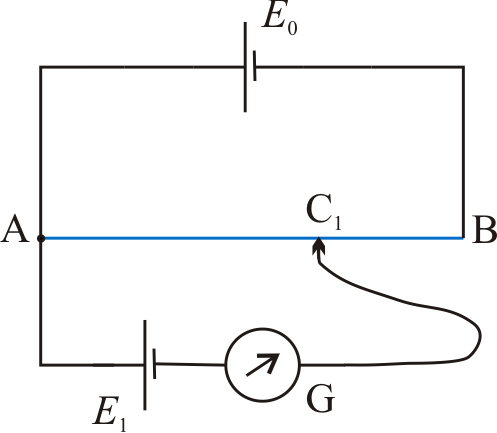
\includegraphics[width=0.4\textwidth]{potentiometer}
	\end{figure}
	When the galvanometer shows zero deflection, i.e. no current passes through $G$, the emf of $E_1$ can be found by:
	\begin{equation*}
	V_{E_1} = \frac{L_{\text{AC$_1$}}}{L_{\text{AB}}} \times V_{E_0}
	\end{equation*}
	To find the internal resistance of $E_1$, a resistor of known resistance is added across $E_1$, and the position of $C_1$ adjusted such that the galvanometer again shows no deflection. This effectively creates two separate circuits, one around $E_0AB$ and one from $E_1$ to the resistor. The terminal potential difference of $E_1$ can be found using the same equation as above. Using this value, the previously found electromotive force of $E_1$, and the potential divider rule, the internal resistance can be found accordingly. 
	
	\newpage
	\section{EM and EMI}
	\subsection{Concepts}
	\begin{center}
		\renewcommand{\arraystretch}{1.2}
		\begin{tabular}{@{} l l p{8.6cm} @{}}
			\toprule
			Magnetic Flux Density & $B$ & The \textbf{force per unit length per unit current} acting on an \textbf{infinitely long} current carrying conductor placed perpendicular to the magnetic field. The SI unit is the tesla, \si{\tesla}. \\
			$\rightarrow$ Tesla & \si{\tesla} & The magnetic flux density of a magnetic field is said to be \SI{1}{\tesla} if the force acting per unit length on an infinitely long conductor carrying a current of \SI{1}{\ampere} and placed perpendicular to the magnetic field is \SI{1}{\newton\per\meter}. \\
			Magnetic Flux & $\varphi=\textbf{B}\cdot\textbf{A}$ & The magnetic flux through a surface is the product of the magnetic flux density \textbf{normal} to the surface and the area of the surface. The SI unit is the weber, \si{\weber}. \\
			$\rightarrow$ Weber & \si{\weber} & The weber is defined as the magnetic flux through a surface of \SI{1}{\meter\squared} if a magnetic field of flux density \SI{1}{\tesla} exists perpendicular to the surface.\\
			Flux Linkage & $\Phi=N\textbf{B}\cdot\textbf{A}$ & The product of the magnetic flux through a coil and the number of turns of the coil. The SI unit is also the weber, \si{\weber}. \\
			\midrule
			Lenz's Law & \multicolumn{2}{p{11.1cm}}{The polarity of the induced EMF is such that it tends to produce a current that creates a magnetic field so as to oppose the change in magnetic flux. It is a statement of the conservation of energy where the mechanical energy is converted to electrical energy. This law allows us to determine the polarity of the induced EMF and predict the direction of the induced current.} \\
			\bottomrule
		\end{tabular}
	\end{center}
	\subsection{Equations}
	\begin{center}
		\renewcommand{\arraystretch}{1.2}
		\begin{tabular}{@{} l l @{}} %C{9cm}
			\toprule
			Force on Current Carrying Conductor & $\textbf{F} = \textbf{I}L\times\textbf{B}$\\
			Force on Moving Charge & $\textbf{F} = q\textbf{v}\times\textbf{B}$\\
			Torque in DC Motor & $\tau = NBIA\sin\theta$\\
			Faraday's Law & $\varepsilon \propto \frac{d\Phi}{dt}$\\
			Induced EMF in AC Generator & $\varepsilon = NBA\omega\sin\left(\omega t\right)$\\
			Induced EMF in a Rod Cutting Flux & $\varepsilon = B_\perp Lv$\\
			Induced EMF in a Faraday's Disc & $\varepsilon = BAf$\\
			\bottomrule
		\end{tabular}
	\end{center}
	\section{Alternating Current}
	\begin{center}
		\renewcommand{\arraystretch}{1.8}
		\begin{tabular}{@{} l p{9.5cm} @{}}
			\toprule
			Alternating Current & Occurs when charge carriers periodically reverse their direction of motion.\\
			Root-Mean-Square & To find the RMS value for any AC graph: \begin{enumerate}
				\item Square the $I/t$ or $V/t$ graph.
				\item Find area under graph in 1 period.
				\item Divide the area by 1 period.
				\item Square root the above result.
			\end{enumerate}\par
			$$\sqrt{\frac{f(t)^2}{T}}$$
			\par
			If the graph is sinusoidal, the RMS value can be found by simply dividing the peak value by $\sqrt{2}$. The RMS value of an alternating current is the equivalent constant DC that will dissipate the same power in a given resistive load.\\
			AC to DC Conversion & Called rectification. Can be accomplished by placing a diode next to the AC source.\\
			Non-Ideality in Transformers & Caused by:
			\begin{enumerate}
				\item Energy dissipated as heat due to resistance of windings in coils. Can be minimised by using thick coils. 
				\item Alternating magnetic flux induces eddy currents in iron core and causes heating. Can be minimised by using a laminated core.
				\item Hysteresis loss whenever direction of magnetic flux is reversed causing some energy wastage. Can be minimised by using a soft iron core.
				\item Flux leakage if core is badly designed.
			\end{enumerate}\\
			\bottomrule
		\end{tabular}
	\end{center}
	\newpage
	\section{Quantum Physics}
		\subsection{Photoelectric Effect}
			\begin{center}
				\renewcommand{\arraystretch}{1.8}
				\begin{tabular}{@{} l p{10.3cm} @{}}
					\toprule
					$hf=\Phi+KE_{max}$ & The \textit{Photoelectric Effect} is the liberation of electrons from a metal surface when EM radiation of sufficiently high frequency is incident on it. This provides evidence of the particulate nature of EM radiation. $$KE_{max}=\frac{1}{2}mv_{max}^2=eV_{s}$$ \vspace*{-\baselineskip}\\
					Work Function Energy $\Phi$ & The minimum amount of energy needed to remove an electron from a metal surface. This varies with the metal.\\
					Stopping Potential $V_s$ & The minimum pd between the emitter and the collecter that will prevent even the most energetic photoelectrons from reaching the collector. \\
					\bottomrule
				\end{tabular}
			\end{center}
		\subsection{Line Spectra}
			Line Spectra provides the evidence for the existence of \textbf{discrete} energy levels in the atom (interactions with the outermost electrons).
			
			\textit{Conditions of the experiment:}
			\begin{itemize}
				\item Atoms sufficiently isolated so that they do not interact with one another and the energy level remain discrete.
				\item Low-pressure gas is needed.
			\end{itemize}
			
			\begin{center}
				\renewcommand{\arraystretch}{1.8}
				\begin{tabular}{@{} l p{10.9cm} @{}}
					\toprule
					Emission Spectrum & Bright coloured lines on dark background. \par This is due to the photons produced when de-excitation takes place from a higher to a lower energy state. \\
					Absorption Spectrum & Dark lines on bright coloured (rainbow) background. \par Only frequencies corresponding to the difference between energy intervals can be absorbed.\\
					\bottomrule
				\end{tabular}
			\end{center}
		\newpage
		\subsection{X-Ray Spectra}
			X-Ray Spectra is produced due to energy changes in electrons close to the nucleus of metal atoms.
			
			\begin{center}
				\renewcommand{\arraystretch}{1.8}
				\begin{tabular}{@{} p{3.5cm} p{10.5cm} @{}}
					\toprule
					Characteristic Lines & Peaks resulting as a result of photons emitted from outer shell electrons falling into vacancies in the inner shells (e.g. L $\rightarrow$ K). The positions of the peaks depend solely on the type of metal. \par $\Rightarrow$ Energy differences in the inner shells are large $\Rightarrow$ shorter $\lambda$\\
					Continuous Radiation (Bremsstrahlung) & Result of the loss in KE when the energetic bombarding electrons decelerate as they hit the metal target. The photon has $\lambda_{min}$ when all the KE of the electron is converted to energy in the form of a photon. $$hf_{max}=\frac{hc}{\lambda_{min}}=eV$$ \vspace*{-\baselineskip}\\
					\bottomrule
				\end{tabular}
			\end{center}
		\subsection{Wave-Particle Duality}
			Waves can exhibit particle-like characteristics and particles can exhibit wave-like characteristics.
			
			$$\textrm{de Broglie wavelength }\lambda = \frac{h}{p}=\frac{h}{mv}$$
		\subsection{Heisenberg's Uncertainty Principle}
			\begin{center}
				\renewcommand{\arraystretch}{1.8}
				\begin{tabular}{@{} p{3.5cm} l p{8.3cm} @{}}
					\toprule
					Position-Momentum Uncertainty Principle & $\displaystyle \Delta x \Delta p \geq \frac{h}{4\pi}$ & If a measurement of position of a particle is made with uncertainty $\Delta x$ and a simultaneous measurement of linear momentum is made with uncertainty $\Delta p$, then the product of the 2 uncertainties can never be smaller than $\frac{h}{4\pi}$. \\
					Energy-Time Uncertainty Principle & $\displaystyle \Delta E \Delta t \geq \frac{h}{4\pi}$ & $\Delta E$ is the uncertainty in the energy of the system, and $\Delta t$ is the time during which the system exists unperturbed. Definition is similar to that of the one above. \par Linewidth is a result of this uncertainty principle. \\
					\bottomrule
				\end{tabular}
			\end{center}
		\subsection{Schr\"{o}dinger Model and Wave Function}
			The wave function $\Psi$ is obtained when one solves the Schr\"{o}dinger equation.
			\begin{center}
				\renewcommand{\arraystretch}{1.6}
				\begin{tabular}{@{} p{3.4cm} p{10.9cm} @{}}
					\toprule
					Significance of the wave function $\Psi$ & $|\Psi|^2$ is the probability density function (of finding the particle). Hence, the probability of find the particle between $x=a$ and $x=b$ is given by $$\int_{a}^{b}|\Psi|^2 dx$$\vspace*{-\baselineskip}\\
					Quantum Tunnelling & Classically, a particple of total energy $E$ indicent on potential energy barrier $U$, where $U>E$, will not be able to cross the barrier, since that would mean that the particle has negative KE when it is crossing the barrier. \par However, when one solves the Schr\"{o}dinger equation to obtain the particle's wave function $\Psi$, one realizes that there is a probability of finding the particle on the other side of the barrier.$$T \propto e^{-2kd}~,~~\textrm{where } k=\sqrt{\frac{8\pi^2m(U-E)}{h^2}}$$ \vspace*{-\baselineskip}\\
					\bottomrule
				\end{tabular}
			\end{center}
	\section{Lasers and Semiconductors}
	\begin{center}
		\renewcommand{\arraystretch}{1.8}
		\begin{tabular}{@{} l p{10cm} @{}}
			\toprule
			Spontaneous Emission & Emission of photons through random de-excitation of excited atoms. These photons are of random phase, direction and plane of polarisation.\\
			Stimulated Emission & Emission of photons from excited atoms as triggered by an incident photon with energy exactly equal to the difference between the excited state and the lower energy state. Emitted photon has exactly the same phase, energy, polarisation and direction of travel as incident photon.\\
			Population Inversion & Condition where there are more atoms in the upper energy state/level than in the lower energy state/level.\\
			Metastable State & Excited state with longer life-time than other excited states.\\
			Conduction Band & Empty or partially filled band just above the valence band.\\
			Valence Band & Highest \textbf{fully-filled} energy band at \SI{0}{\kelvin}.\\
			Metals & Metals have a partially filled conduction band at \SI{0}{\kelvin}.\\
			Insulators & Insulators have a fully-filled valence band and empty conduction band at 0K, and also a large bandgap. There are very few electrons in the conduction band even at room temperature due to the large bandgap.\\
			Intrinsic Semiconductor & Intrinsic semiconductors have a full valence band and empty conduction band at 0K, but a smaller bandgap than that of insulators. An appreciable number of electrons are promoted to the conduction band at room temperature due to the smaller bandgap.\\
			\bottomrule
		\end{tabular}
	\end{center}
	\newpage
	\section{Nuclear Physics}
	\begin{center}
		\renewcommand{\arraystretch}{1.25}
		\begin{tabular}{@{} l p{10cm} @{}}
			\toprule
			Nucleon & A constituent of a nucleus, i.e. a proton or neutron.\\
			Nuclide & A \textbf{species} of atom characterised by \textbf{constituent of nucleus} (no. of neutrons and protons).\\
			Isotope & Atoms with the same number of protons but different number of neutrons.\\
			Unified Atomic Mass Unit & 1 u is defined as $\frac{1}{12}$ of the mass of a Carbon-12 atom.\\
			Binding Energy of Nucleus/Atom & The energy required to \textbf{separate} the nucleus/atom into its \textbf{constituents}.\\
			Binding Energy per Nucleon & The \textbf{average} energy required to remove a nucleon from its nucleus.\\
			Radioactive Decay & A \textbf{spontaneous} and \textbf{random} process where an \textbf{unstable} nucleus changes into a different nuclide by emitting radiation. Spontaneous means that it is not triggered by external factors or influences, and random means that it is impossible to predict \textbf{which} nucleus will decay and \textbf{when} a \textbf{particular} nucleus will decay.\\
			Activity & The rate of decay, or number of disintegrations per unit time. SI unit is \si{\per\second} or the becquerel, \si{\becquerel}. $$A = -\frac{dN}{dt} = \lambda N$$ \vspace*{-\baselineskip}\\
			Decay Constant & \textbf{Probability per unit time} that a nucleus will decay. SI unit is \si{\per\second}. $$\lambda = \frac{A}{N}$$ \vspace*{-\baselineskip}\\
			Half-Life & The \textbf{average} time taken for a number of \textbf{radioactive} nuclei to decay to \textbf{half} its original value. $$t_{\frac{1}{2}} = \frac{\ln 2}{\lambda}$$ \vspace*{-\baselineskip}\\
			\bottomrule
		\end{tabular}
	\end{center}
	\vspace{2cm}
	\begin{center}
		{\LARGE That's all folks!}
		
		{\huge Good luck! Don't panic, all is well.}
	\end{center}
\end{document}
